% \section{Side by side comparison}
% \label{sec:comparison}

% In this section we compare both results side by side. Firstly, the output of the envelope detector (take note that the theoritcal analysis one is the plot in orange):
% \begin{figure*}[h]
%     \centering
%     \begin{subfigure}{0.23\textwidth}
%         \includegraphics[width=\linewidth, clip]{gainACtotal.eps}
%         \label{fig:envd1}
%     \end{subfigure}
%     \begin{subfigure}{0.23\textwidth}
%         \includegraphics[width=\linewidth, clip]{gainACtotal.eps}
%         \label{fig:envd2}
%     \end{subfigure}
%     \caption{\small Gain Stage......Comparison}
%     \label{env_detector}
% \end{figure*}

% % \begin{figure}[h]
% %     \centering
% %     \begin{subfigure}{0.23\textwidth}
% %         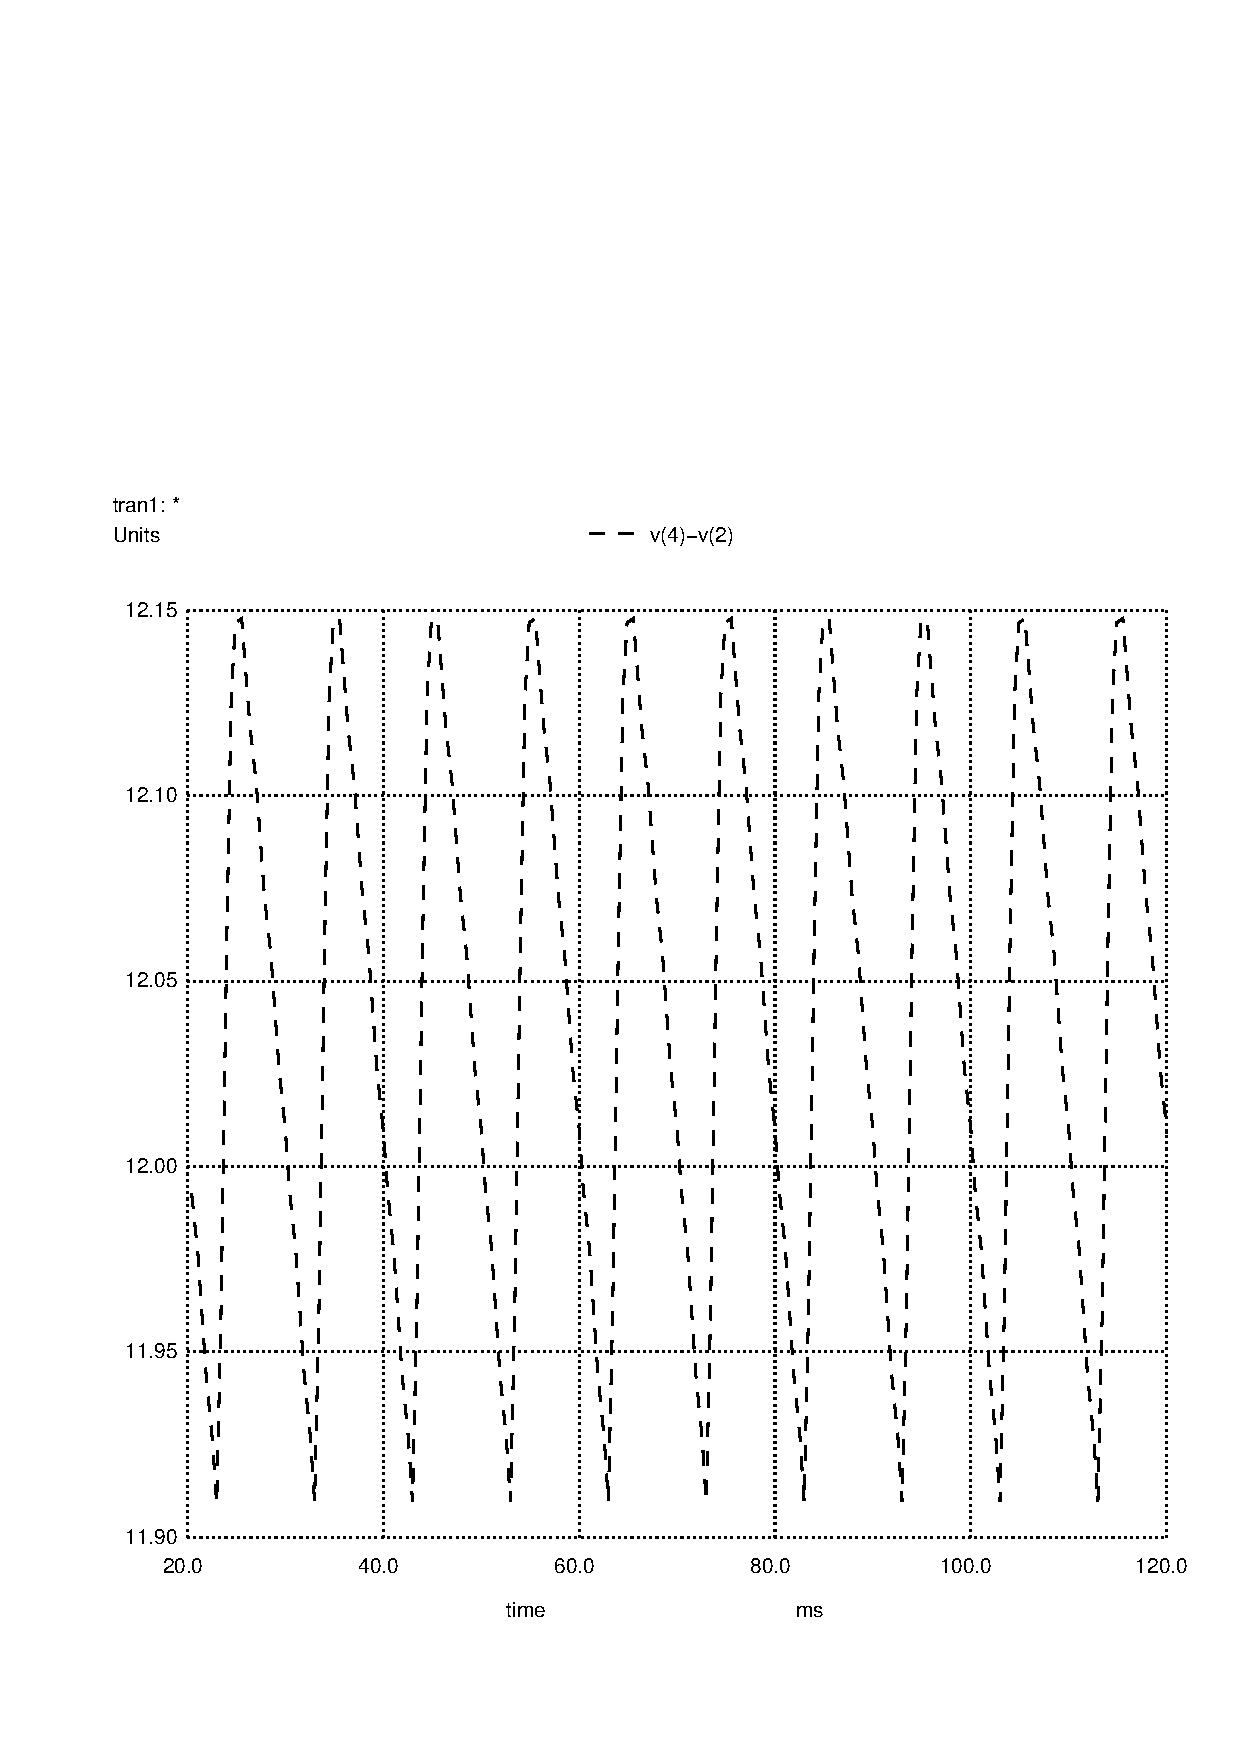
\includegraphics[width=\linewidth, clip]{solution1.pdf}
% %         \label{fig:voltr1}
% %     \end{subfigure}
% %     \begin{subfigure}{0.23\textwidth}
% %         \includegraphics[width=\linewidth, clip]{voltageRegulator.eps}
% %         \label{fig:voltr2}
% %     \end{subfigure}
% %     \caption{\small Voltage regulator output (left - simulation; right - theoretical )}
% %     \label{volt_reg}
% % \end{figure}

% The shape of the graphs, both envelope detector and voltage regulator is similar, so we can concluse that both fullfill their purposes and the theoretical model used was good at predicting the general behaviour of the circuit.
% However, especially on the voltage regulator graphs, we can see some differences in the scale of the oscillations, that can be due to the different models used in our theoretical simulation, compared to ngspice.
% We can quantify this diffetence with the values of the ripples.

% \begin{figure}[h]
%     \centering
%     \begin{subfigure}{0.23\textwidth}
%         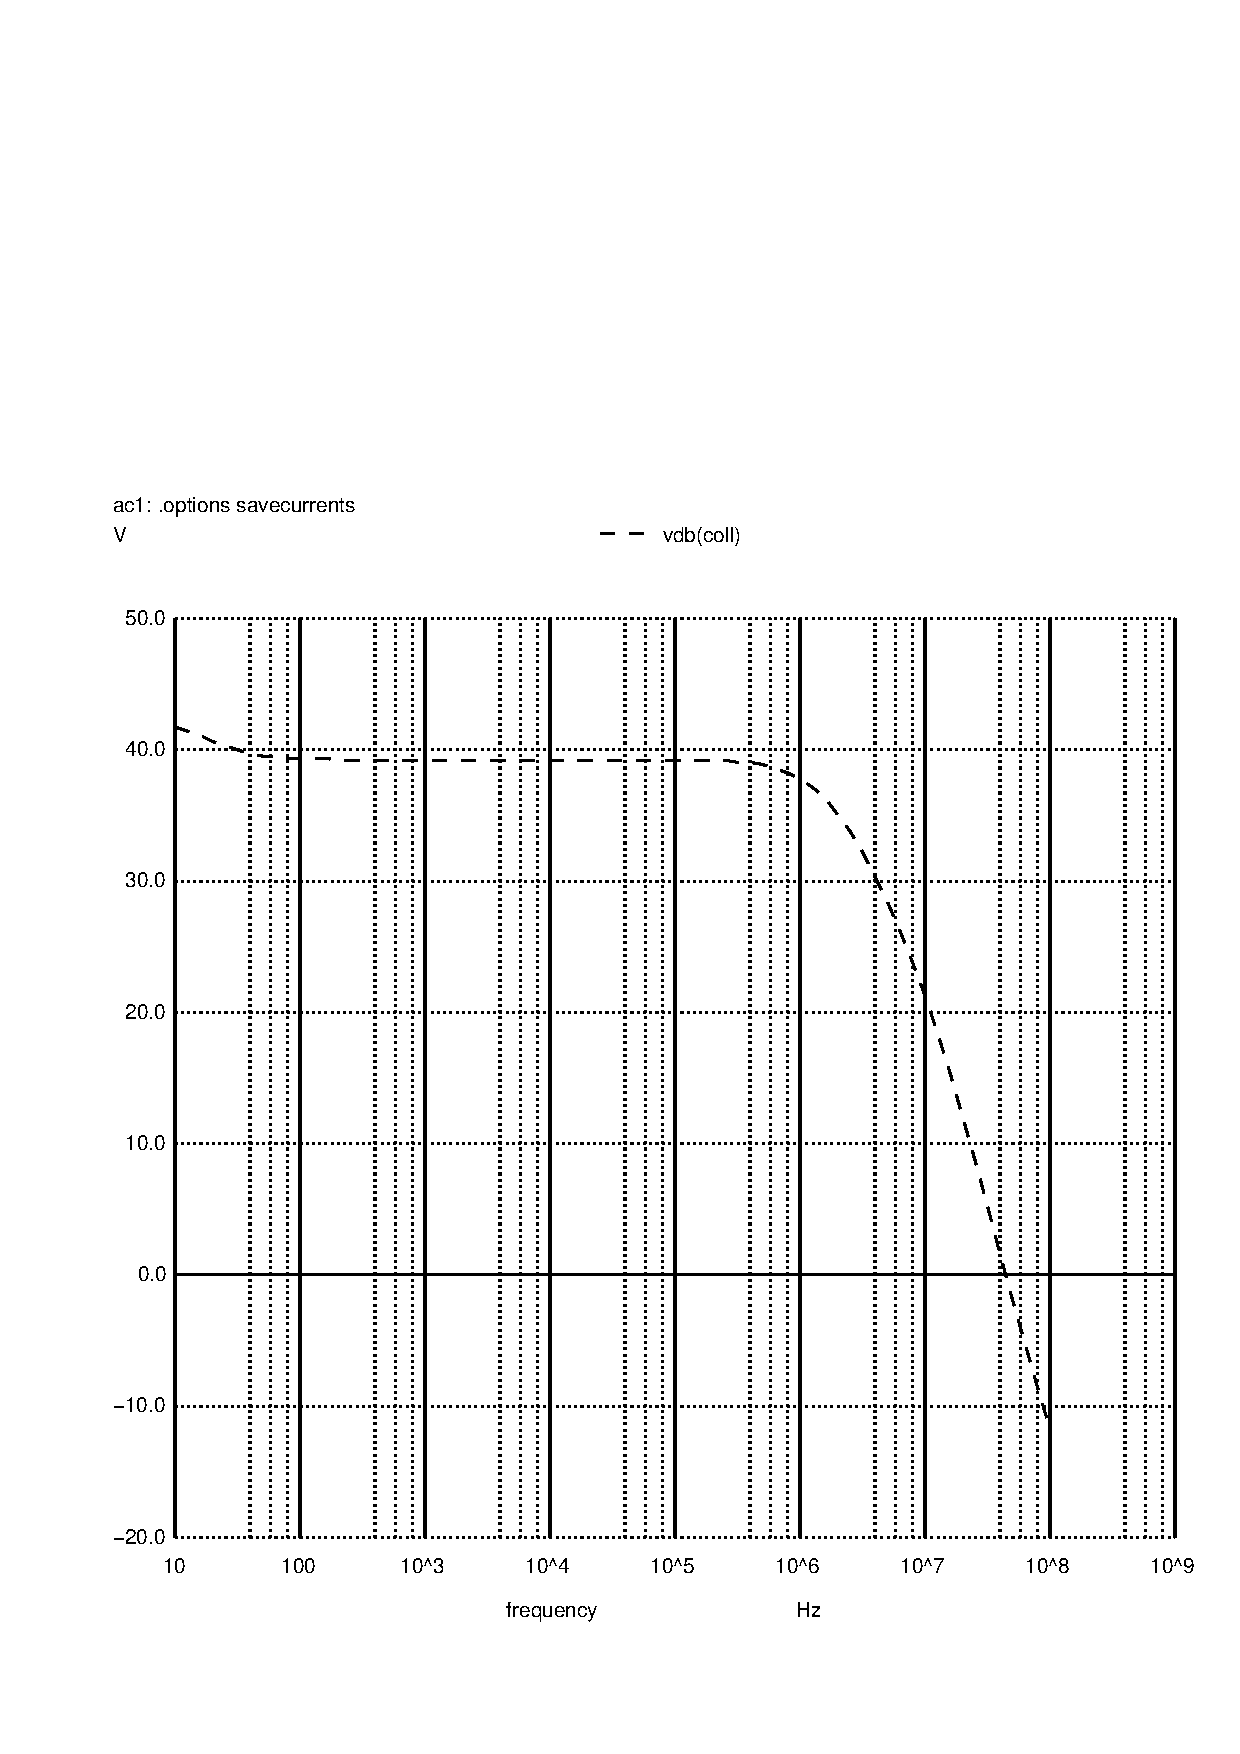
\includegraphics[width=\linewidth, clip]{vo2f.pdf}
%         \label{fig:output1}
%     \end{subfigure}
%     \begin{subfigure}{0.23\textwidth}
%         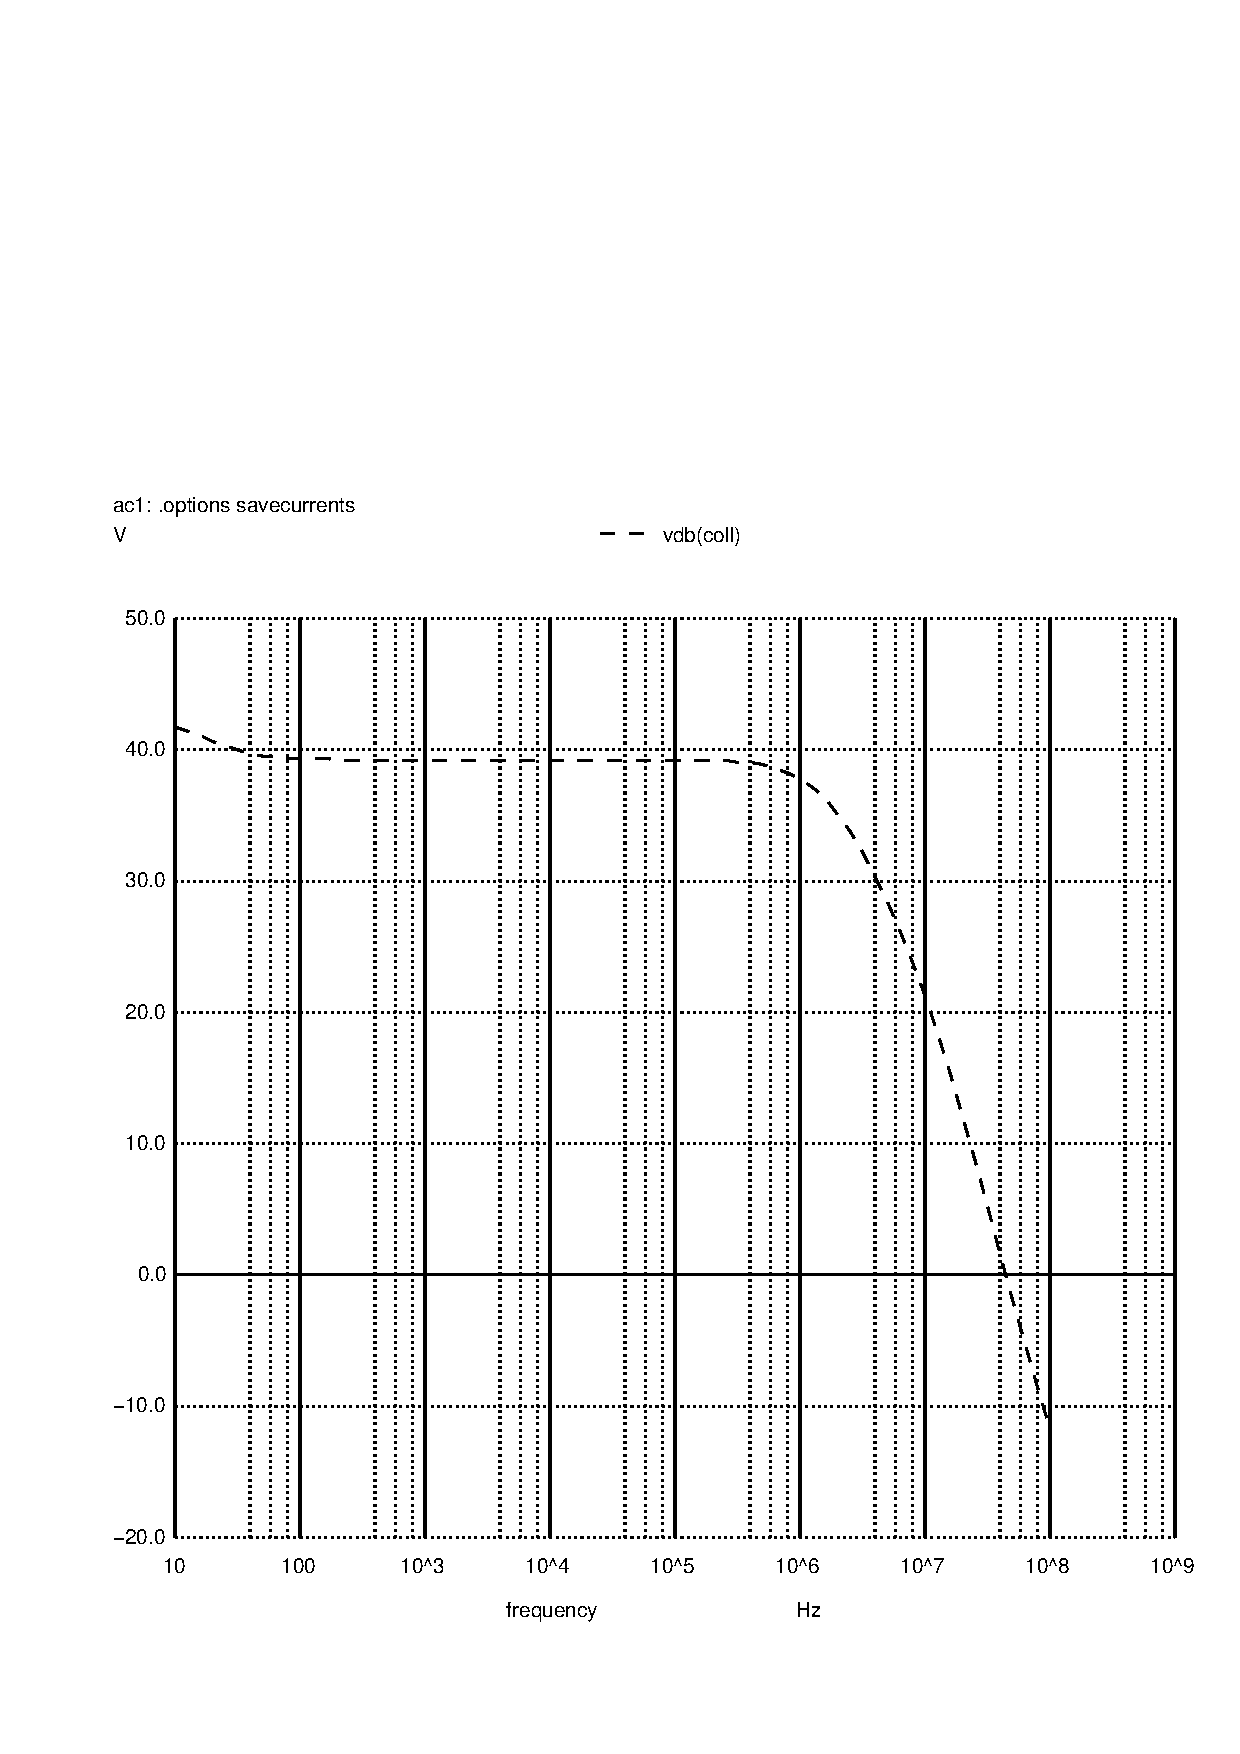
\includegraphics[width=\linewidth, clip]{vo1f.pdf}
%         \label{fig:output2}
%     \end{subfigure}
%     \caption{\small $V_Out - 12$ - measure of the output DC deviation + AC component (left - simulation; right - theoretical )}
%     \label{output_deviation}
% \end{figure}

% \begin{table}
%     \parbox{.45\linewidth}{
%         \centering
%         \begin{tabular}{|c|c|}
%             \hline
%             {\bf Name} & {\bf Value [A or V]} \\ \hline
%             gm1 & 3.577156e-01\\ \hline
$r pi 1$ & 4.995588e+02\\ \hline
r01 & 7.793900e+03\\ \hline
AV1 & -2.627909e+02\\ \hline
$AV1_{DB}$ & 4.839221e+01\\ \hline
ZI1& 4.844336e+02\\ \hline
ZO1 & 8.862848e+02\\ \hline

%         \end{tabular}
%         \label{tab:GainStage_AC}
%         \caption{Results of Nodal Analysis of the circuit for t < 0. A variable that begins  with \textit{I} names a \textit{current} in \textit{Ampere}; the ones that start with \textit{V} name a \textit{voltage} in \textit{Volt}}
%     }
%     \hfill
%     \parbox{.45\linewidth}{
%         \centering
%         \begin{tabular}{|c|c|}
%             {\bf Name} & {\bf Value [A or V]} \\ \hline
%             VEQ & 2.400000e+00\\ \hline
IB1 & 5.004416e-05\\ \hline
IC1 & 8.942891e-03\\ \hline
VEQ & 8.992935e-03\\ \hline
VE1 & 8.992935e-01\\ \hline
V01 & 3.057109e+00\\ \hline
VCE & 2.157816e+00\\ \hline

%             \hline
%         \end{tabular}
%         \label{tab:GainStage_OP}
%         \caption{Table with results from Ngspice to find out the voltages and currents in each node and branch. A variable that begins  with \textit{I} names a \textit{current} in \textit{Ampere}; the ones that start with \textit{V} name a \textit{voltage} in \textit{Volt} }
%     }
% \end{table}

% Once again, as in the previous graphs, the output deviation graph has a similar shape but a noticeable difference in scale, probably due to different models.


% \begin{center}
%     \begin{tabular}{ |c|c|c| }
%         \hline

%                & Simulation & Theoretical \\
%         Ripple & 0.2391470  & 0.38944     \\

%         \hline
%     \end{tabular}
% \end{center}

% Thus we have obtained a 62\% error in the theoretical ripple. Which is a
% good indicator of the difference between the models used.

\section{Conclusion}
\label{sec:conclusion}


The ultimate goal of this laboratory assignment, to create an audio amplifier 
circuit, has been achieved.
The discrepancies observed between the simulation and theoretical results, 
as described in the side-by-side comparison, were expected.
These can be explained by the fact that the models used to describe the 
components of the circuit, namely the transistors, in \textit{Ngspice} 
and in the theoretical analysis (\ref{sec:analysis}) are extremely 
different. Better results could have been obtained if other models 
for the behaviour of the transistors were used, for instance, the 
transistor with capacitors.


%\lipsum[1-1]
